\chapter{Prediction of the world's temperature}
\label{chap:two}

This chapter outlines several regression models, namely \textit{Polynomial Regression}, \textit{Ridge Regression}, and \textit{Lasso Regression} that are utilized to forecast the Earth's temperature in the current century. Additionally, machine learning models will consider three different scenarios.
\begin{enumerate}
  \item \coo\ emission remains the same as in 2021
  \item \coo\ emission drops yearly by 2\%
  \item \coo\ emission increases yearly by 2\%
\end{enumerate}
Figure ~\ref{fig:cumulative-co2-temperature} demonstrates correlation between normalized\footnote{Normalization is a common technique used for machine learning models. It helps avoid numerical issues during trainning phase and improves stability of some algorithms. } values of \coo\ emission and temperature anomalies.
It is noteworthy that all models used in the experiment uses a \textit{cumulative} function of carbon dioxide emissions, whereby the total amount of emissions is accumulated, as opposed to measuring discrete values on a yearly basis. 
The \textit{cumulative} approach eliminates issues related to non-uniform \coo\ emissions on an annual basis, and furthermore incorporates a historical perspective on emissions.
It is worth to mention that models used for temperature predictions do not take into account absorbtion of \coo\ by forests that provide \textit{carbon sink}. It is estimated that forests can absorb 7.6 billion metric tonnes of \coo\ per year\cite{forest-absorbs} that is unfortunately only 3.5\% of 2021's \coo\ emission.
On the other hand recent findings\cite{forest-emits}, discovered that Amazon rainforets emits now more \coo\ that it can absorbe and it has become a source of \coo\, rather than a sink. It appears that there is a need for further research and improved data quality and understanding in the field of climate change. 

\begin{figure}[h]
  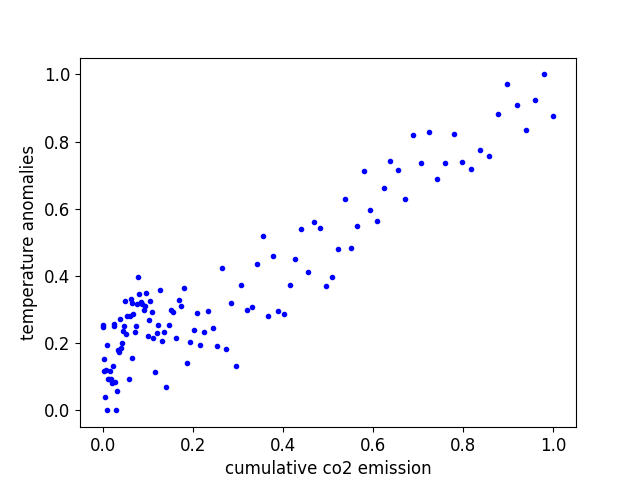
\includegraphics[width=\linewidth]{img/cumulative-co2-temperature.png}
  \caption{TODO}
  \label{fig:cumulative-co2-temperature}
\end{figure}

\newpage
\section{Linear Regresion}
Result of \textit{Linear Regression} method are demonstrated on ~\ref{fig:linear-regression}. Line that approxymates the model is described by formula:
\[ y = 0.14551849x + 0.7704561  \]
Despite achieving a high coefficient of determination score of 0.86, the Linear Regression model will not be utilized for predicting Earth's temperature.
The following section of the chapter explores more advanced regression methods.
\begin{figure}[h]
  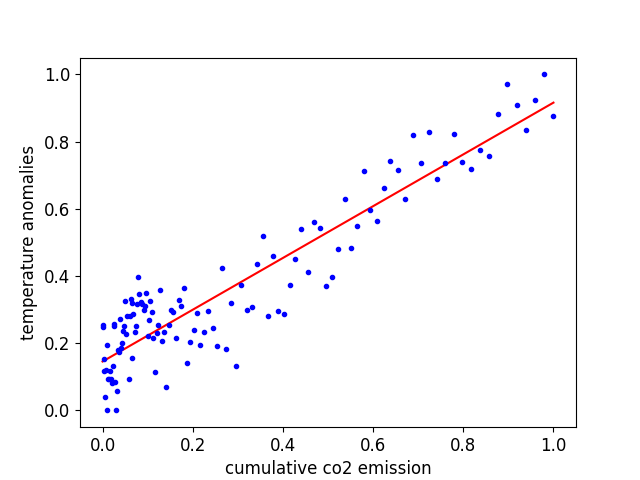
\includegraphics[width=\linewidth]{img/linear-regression.png}
  \caption{Linear Regression model used for temperature anomalies prediction }
  \label{fig:linear-regression}
\end{figure}

\newpage
\section{Polynomial Regression}
Result of \textit{Polynomial Regression} method are demonstrated on ~\ref{fig:polynomial-regression}. Coefficient of determination score equals 0.87 and it is sligtly higher than \textit{Linear Regression}
Interesting result are visible on ~\ref{fig:polynomial-regression-result}, where three different scenarios were take into account. In all cases increases of temperature is inevitable. 
\begin{figure}[h]
  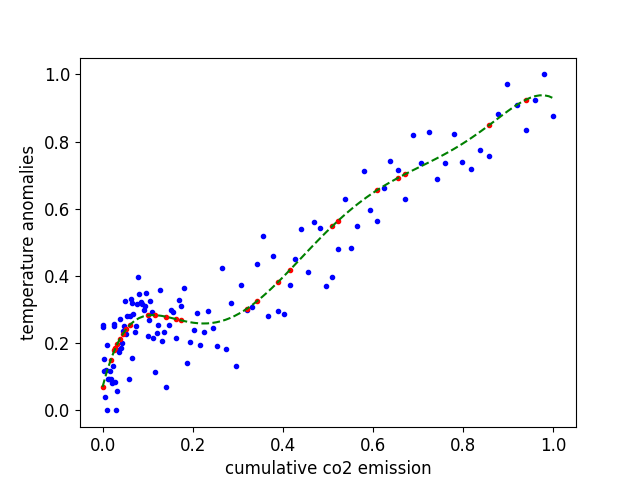
\includegraphics[width=\linewidth]{img/polynomial-regression.png}
  \caption{Polynomial Regression model used for temperature anomalies prediction}
  \label{fig:polynomial-regression}
\end{figure}
\begin{figure}[h]
  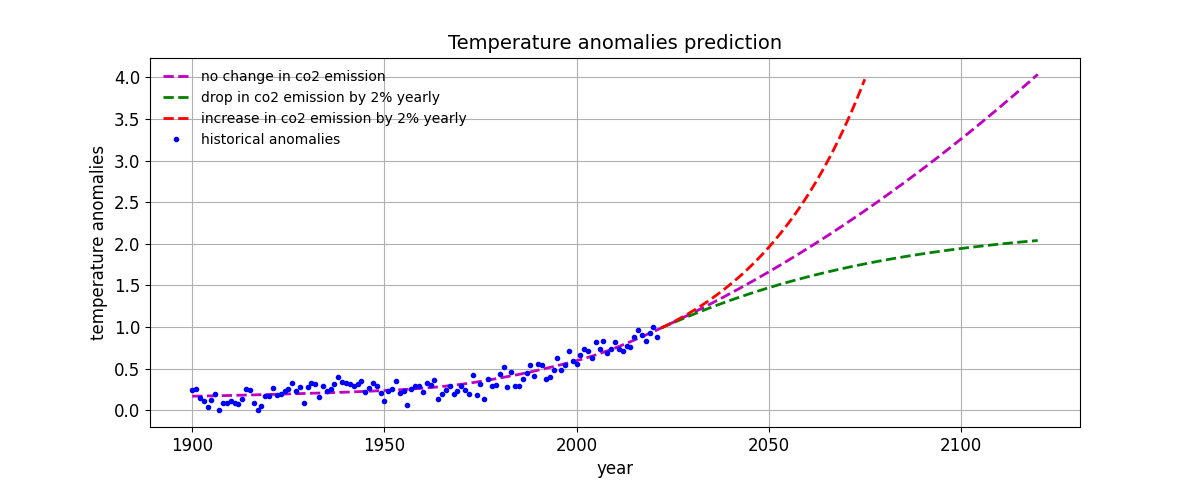
\includegraphics[width=\linewidth]{img/polynomial-regression-result.png}
  \caption{Polynomial Regression model used for temperature anomalies prediction}
  \label{fig:polynomial-regression-result}
\end{figure}
\newline
Based ~\ref{fig:polynomial-regression-result} on we can summary future Earth's temperature in selected years as below ~\ref{fig:polynomial-regression-table}. 
\begin{table}[ht]
\begin{tabular}{ |p{4cm}||p{2cm}|p{2cm}|p{2cm}|  }
 \hline
 & \textbf{2050} & \textbf{2075} & \textbf{2100} \\
 \hline
constant emission &  +2.16\degree C	& +3.11\degree C 	& +4.23\degree C \\
  drops yearly by 2\% &  +1.91\degree C &	+2.28\degree C &	+2.5\degree C  \\
  increases yearly by 2\% &  +2.54\degree C &	+5.17\degree C &	+11.37\degree C  \\
 \hline
\end{tabular}
\caption{Prediction of Earth's temperature in 2050, 2075 and 2100 using \textit{Polynomial Regression} methods} 
\label{tab:polynomial-regression-table}
\end{table}

\newpage
\section{Ridge Regression}
Result of \textit{Ridge Regression} method are demonstrated on ~\ref{fig:ridge-regression}. Coefficient of determination score equals 0.87 and it is the same as \textit{Polynomial Regression}
Similarly as for previous model we can notice prediction of Earth's temperature as ~\ref{fig:ridge-regression-result}. 
\begin{figure}[h]
  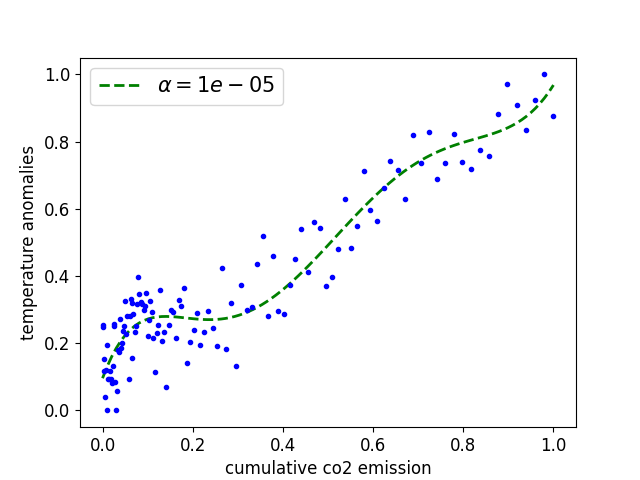
\includegraphics[width=\linewidth]{img/ridge-regression.png}
  \caption{Ridge Regression model used for temperature anomalies prediction}
  \label{fig:ridge-regression}
\end{figure}
\begin{figure}[h]
  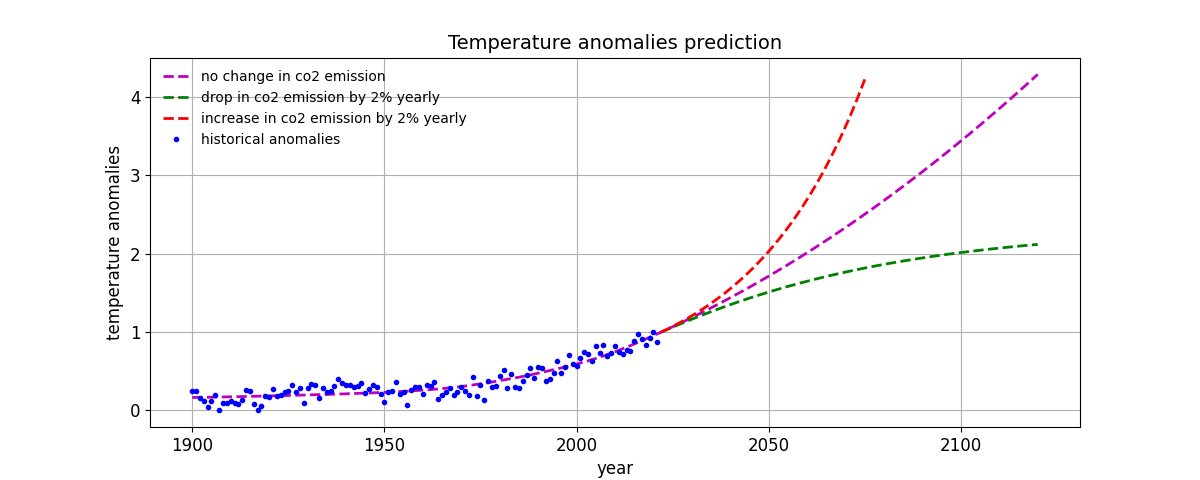
\includegraphics[width=\linewidth]{img/ridge-regression-result.png}
  \caption{Ridge Regression model used for temperature anomalies prediction}
  \label{fig:ridge-regression-result}
\end{figure}
We can calulate ~\ref{fig:ridge-regression-result}. 
\begin{table}[ht]
\begin{tabular}{ |p{4cm}||p{2cm}|p{2cm}|p{2cm}|  }
 \hline
 & \textbf{2050} & \textbf{2075} & \textbf{2100} \\
 \hline
constant emission &  +2.22\degree C	& +3.25\degree C 	& +4.46\degree C \\
  drops yearly by 2\% &  +1.96\degree C &	+2.36\degree C &	+2.61\degree C  \\
  increases yearly by 2\% &  +2.54\degree C &	+5.17\degree C &	+11.37\degree C  \\
 \hline
\end{tabular}
\caption{Prediction of Earth's temperature in 2050, 2075 and 2100 using \textit{Ridge Regression} methods} 
\label{tab:ridge-regression-table}
\end{table}

\newpage
\section{Lasso Regression}

\begin{figure}[h]
  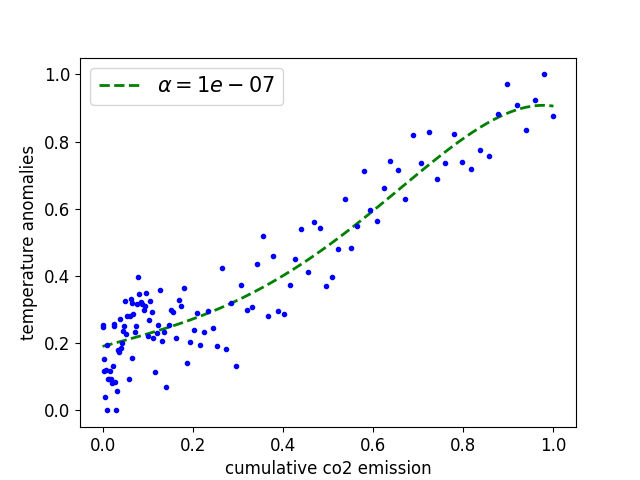
\includegraphics[width=\linewidth]{img/lasso-regression.png}
  \caption{Lasso Regression model used for temperature anomalies prediction}
  \label{fig:lasso-regression}
\end{figure}

\newpage
\section{Gausian Process}

\begin{figure}[h]
  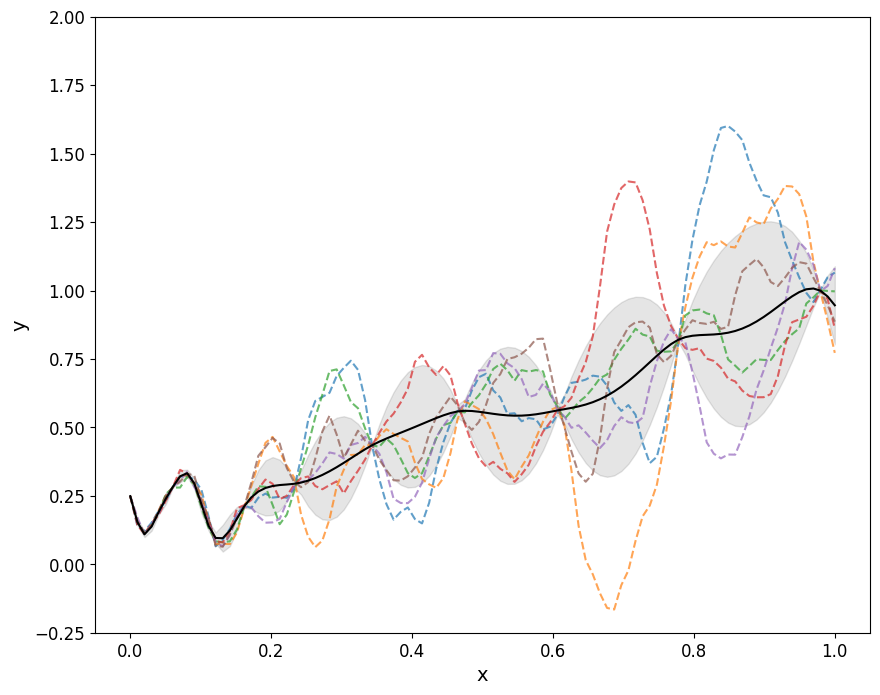
\includegraphics[width=\linewidth]{img/gaussian-process.png}
  \caption{Gaussian Process model used for temperature anomalies prediction}
  \label{fig:gaussian-process}
\end{figure}

\section{Comparision of ML algorithms}

\section{Summary}
